\documentclass[12pt]{article}
\usepackage[utf8]{inputenc}

%% preambleb
\usepackage{amsmath}
\usepackage[margin = 1in]{geometry}
\usepackage{graphicx}
\usepackage{booktabs}
\usepackage{amsthm}
\usepackage{hyperref}
\usepackage{natbib}
\usepackage{enumitem}
\usepackage{setspace}

%% metadata
\title{LaTeX Paper Template}
\author{Ginamarie Mastrorilli\\
    University of Connecticut
}
\date{September 26, 2022}

\begin{document}
\maketitle

\begin{abstract}
write abstract here
\end{abstract}


\section{Introduction}
\label{sec:intro}

Use this section to answer three questions:
Why is the topic important/interesting?
What has been done on this topic in the literature?
What is your contribution?


\section{Data}
\label{sec:data}

Use this section to describe the data that helps to answer your research questions.




\section{Methods}
\label{sec:meth}

Use this section to present the methodologies that will generate results by
analyzing the data. 

Suppose that the radius of a circle is $r$. Then its area is
\begin{equation}
  \label{eq:area}
  \pi r^2.
\end{equation}

Equation~\eqref{eq:area} is something silly.

Sometimes I don't want an equation to be numbered such as this one:
\[
  f(x) = \frac{1}{\sqrt{2\pi}} \exp\left( - \frac{x^2}{2} \right),
\]
which is the density of a standard normal variable.



\section{Results}
\label{sec:results}

Table~\ref{tab:rv} summarizes some example draws from some distributions.

\begin{table}[ht]
  \caption{This is my first table.}
  \label{tab:rv}
\centering
\begin{tabular}{rrr}
  \hline
normal & poisson & gamma \\ 
  \hline
-0.110 & 4 & 2.401 \\ 
  0.116 & 4 & 3.529 \\ 
  -0.828 & 9 & 2.112 \\ 
  -0.066 & 6 & 11.104 \\ 
  0.219 & 3 & 4.815 \\ 
  0.303 & 5 & 2.188 \\ 
  0.544 & 0 & 8.050 \\ 
  -2.617 & 8 & 3.646 \\ 
  0.747 & 1 & 5.178 \\ 
  -1.103 & 4 & 3.043 \\ 
   \hline
\end{tabular}
\end{table}

Figure~\ref{fig:cars} shows the distance against the speed from this dataset.


\begin{figure}
  \centering
  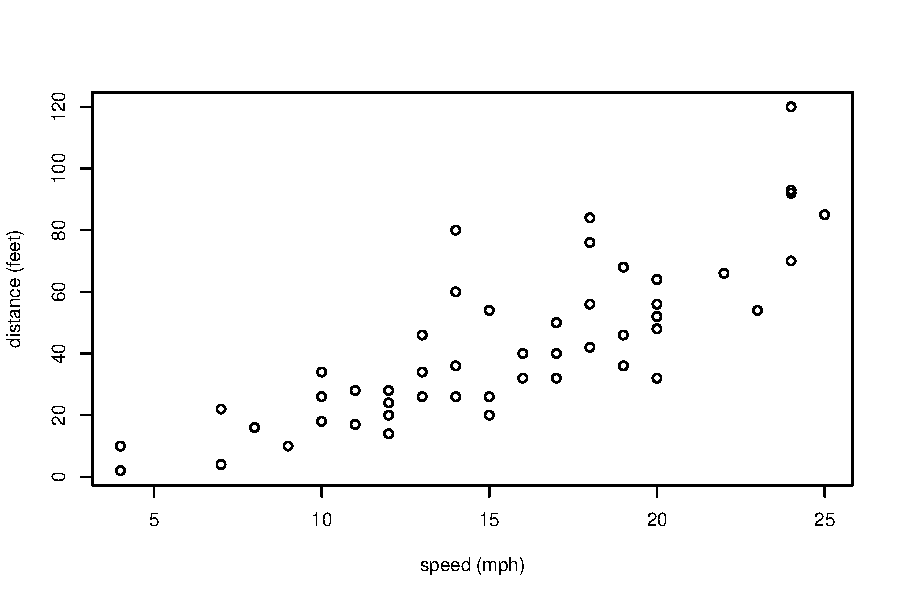
\includegraphics[width=\textwidth]{cars.pdf}
  \caption{This is my first figure.}
  \label{fig:cars}
\end{figure}

\section{Discussion}
\label{sec:disc}

What are the main contributions again?

What are the limitations of this study?

What are worth pursuing further in the future?


\end{document}
